\documentclass{article}
\usepackage{tikz}
\usepackage{amsmath}
\usepackage{svg}
\usepackage{xcolor}
\usepackage[cache=false]{minted}
\usepackage{pdflscape}


\usetikzlibrary {arrows.meta,bending,positioning} 

\usetikzlibrary{shapes.geometric, shapes.arrows}
\usetikzlibrary{patterns}
\usetikzlibrary{quantikz2}
     \tikzset{operator/.append style={fill=white!0}}


\newsavebox{\incode} 
\newsavebox{\fmovecode}
\newsavebox{\fmoveqiskit}
\newsavebox{\nmovecode}
\newsavebox{\nmoveqiskit}



\begin{document}

% Save tabular in a box
\savebox{\fmovecode}{%
    \begin{tabular}{l}
        board[i] = \textcolor{blue}{None} \\ 
        board[i+d1, i+d2] = \{\\
            \quad \textcolor{orange}{'color'} : \textcolor{blue}{red}, \\
            \quad \textcolor{orange}{'probability'} : \textcolor{blue}{0.5}, \\
            \quad \textcolor{orange}{'pawn'} : \textcolor{blue}{1}\} \\
    \end{tabular}
}

\savebox{\incode}{%
\begin{tabular}{l} 
    board[i] = \{\\ 
        \quad \textcolor{orange}{'color'} : \textcolor{blue}{red}, \\ 
        \quad \textcolor{orange}{'probability'} : \textcolor{blue}{1}, \\ 
        \quad \textcolor{orange}{'pawn'} : \textcolor{blue}{1} 
        \} 
    \end{tabular}
}

\savebox{\fmoveqiskit}{%
    \begin{tabular}{l} 
        circuit.cx(q[i], q[i+d1]) \\
        circuit.cx(q[i], q[i+d1]) \\
        circuit.h(q[i+d1]) \\
        circuit.h(q[i+d2]) \\
        circuit.x(q[i])
    \end{tabular}
}

\savebox{\nmovecode}{%
    \begin{tabular}{l}
        board[i] = \textcolor{blue}{None} \\ 
        board[i+d1, i+d2] = \{\\
            \quad \textcolor{orange}{'color'} : \textcolor{blue}{red}, \\
            \quad \textcolor{orange}{'probability'} : $\mathcolor{blue}{(1/2)^n}$, \\
            \quad \textcolor{orange}{'pawn'} : \textcolor{blue}{1}\} \\
    \end{tabular}
}

\savebox{\nmoveqiskit}{%
\begin{tabular}{l} 
    circuit.h(q[i]) \\
    circuit.cx(q[i], q[i+d1]) \\
    circuit.cx(q[i], q[i+d1]) \\
    circuit.h(q[i+d1]) \\
    circuit.h(q[i+d2]) \\
    circuit.x(q[i])
\end{tabular}
}

    \begin{landscape}
        \begin{center}
            \begin{tabular}{||c c c c c||} 
            \hline
            Move name & Move & Python list & Quantum array & Qiskit \\ [0.5ex] 
            \hline\hline
            Initialize & 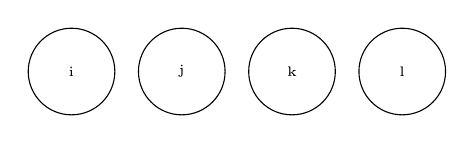
\begin{tikzpicture}
    \def\d{1.4}
    \def\size{1.1}
    \node(c1) [circle, draw, minimum size = \size cm] at (\d * 0,0) {\tiny i};
    \node(c2) [circle, draw, minimum size = \size cm] at (\d * 1,0) {\tiny j};
    \node(c3) [circle, draw, minimum size = \size cm] at (\d * 2,0) {\tiny k};
    \node(c4) [circle, draw, minimum size = \size cm] at (\d * 3,0) {\tiny l};
\end{tikzpicture} & $\text{board=[\textcolor{blue}{None}] * 32}$ & \begin{quantikz}[scale=1.5]
   \lstick{${\ket{0}_i}$} & \\
   \lstick{${\ket{0}_j}$}  &\\
   \lstick{${\ket{0}_k}$}  &\\
   \lstick{${\ket{0}_l}$} &
\end{quantikz} &  \begin{tabular}{l} q = QuantumRegister(10, \textcolor{orange}{'q'}) \\ circuit = QuantumCircuit(q)\end{tabular} \\ [1ex]
            \hline
            New pawn & 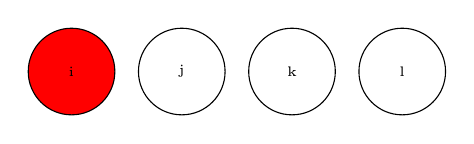
\begin{tikzpicture}
    \def\d{1.4}
    \def\size{1.1}
    \node(c1) [circle, draw, fill=red, minimum size = \size cm] at (\d * 0,0) {\tiny i};
    \node(c2) [circle, draw, minimum size = \size cm] at (\d * 1,0) {\tiny j};
    \node(c3) [circle, draw, minimum size = \size cm] at (\d * 2,0) {\tiny k};
    \node(c4) [circle, draw, minimum size = \size cm] at (\d * 3,0) {\tiny l};
\end{tikzpicture} & \usebox{\incode} & \begin{quantikz}[scale=1.5]
    \lstick{$\ket{0}_i$} & \gate{X} & \rstick{$\ket{1}_i$}\\
    \lstick{$\ket{0}_j$}& &\\
    \lstick{$\ket{0}_k$} &&\\
    \lstick{$\ket{0}_l$} &&\\[-1em]
\end{quantikz} & circuit.x[q[i]] \\
            \hline
            First move & 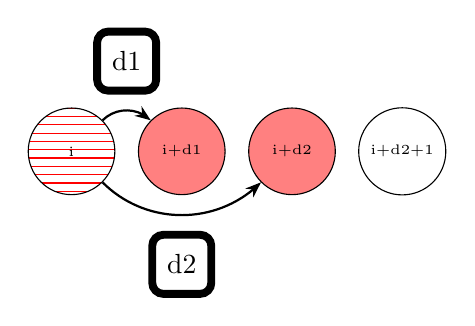
\begin{tikzpicture}
    \def\d{1.4}
    \def\size{1.1}
    \node(c1) [circle, draw, minimum size = \size cm, pattern={horizontal lines},pattern color=red] at (\d * 0,0) {\tiny i};
    \node(c2) [circle, draw, minimum size = \size cm, fill = red!50] at (\d * 1,0) {\tiny i+d1};
    \node(c3) [circle, draw, minimum size = \size cm, fill = red!50] at (\d * 2,0) {\tiny i+d2};
    \node(c4) [circle, draw, minimum size = \size cm] at (\d * 3,0) {\tiny i+d2+1};

    \draw[draw, thick, -{Stealth[length=2mm]}]
    (c1) edge [bend left=45] node[pos=0.5, above, rectangle, draw, minimum width = 0.75 cm, minimum height = 0.75 cm, rounded corners, line width = 0.1 cm, yshift=0.2cm] {d1} (c2)
    (c1) edge [bend right=45] node[pos=0.5, below, rectangle, draw, minimum width = 0.75 cm, minimum height = 0.75 cm, rounded corners, line width = 0.1 cm, yshift=-0.2cm] {d2} (c3);
\end{tikzpicture} & \usebox{\fmovecode} & \begin{quantikz}[color=gray, scale=1]
    \lstick{\small$i\;$} & \setwiretype{q} & \ctrl{1} & \ctrl{2} & \gate{X}& \\
    \lstick{\small$i+d1\;$} & \setwiretype{q} & \targ{ } &          & \gate{H}& \\
    \lstick{\small$i+d2\;$} & \setwiretype{q} &          & \targ{ } & \gate{H}& 
\end{quantikz} & \usebox{\fmoveqiskit} \\
            \hline
            nth move & 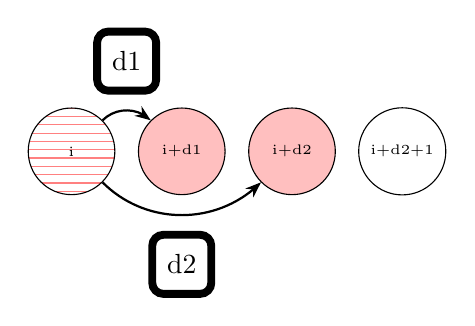
\begin{tikzpicture}
    \def\d{1.4}
    \def\size{1.1}
    \node(c1) [circle, draw, minimum size = \size cm, pattern={horizontal lines},pattern color=red!50] at (\d * 0,0) {\tiny i};
    \node(c2) [circle, draw, minimum size = \size cm, fill = red!25] at (\d * 1,0) {\tiny i+d1};
    \node(c3) [circle, draw, minimum size = \size cm, fill = red!25] at (\d * 2,0) {\tiny i+d2};
    \node(c4) [circle, draw, minimum size = \size cm] at (\d * 3,0) {\tiny i+d2+1};

    \draw[draw, thick, -{Stealth[length=2mm]}]
    (c1) edge [bend left=45] node[pos=0.5, above, rectangle, draw, minimum width = 0.75 cm, minimum height = 0.75 cm, rounded corners, line width = 0.1 cm, yshift=0.2cm] {d1} (c2)
    (c1) edge [bend right=45] node[pos=0.5, below, rectangle, draw, minimum width = 0.75 cm, minimum height = 0.75 cm, rounded corners, line width = 0.1 cm, yshift=-0.2cm] {d2} (c3);
\end{tikzpicture} & \usebox{\nmovecode} & \begin{quantikz}[color=gray, scale=1]
    \lstick{\small$i\;$}  &\gate{H} & \ctrl{1} & \ctrl{2} & \gate{X}& \\
    \lstick{\small$i+d1\;$} &    & \targ{ } &          & \gate{H}& \\
    \lstick{\small$i+d2\;$} &     &       & \targ{ } & \gate{H}& 
\end{quantikz} & \usebox{\nmoveqiskit} \\
            \end{tabular}
        \end{center}
    \end{landscape}
\end{document}
